%% tags: graph network tikzImg polar pac pacLearning aaai aaai19 vcDimension
%% tabular
\documentclass[tikz,border=2]{standalone}
\usetikzlibrary{shadows,arrows,shapes,positioning,calc,backgrounds,fit}
\newcommand{\vanish}[1]{}
\usepackage{array}
\newcommand{\calc}[1]{\mbox{$\mathcal{C}_{#1}$}}
%% \usepackage{ctable}
\pdfpageattr {/Group << /S /Transparency /I true /CS /DeviceRGB>>}
% Define the layers to draw the diagram
%
\begin{document}
%% \pgfdeclarelayer{bg}
%% \pgfdeclarelayer{fg}
%% \pgfsetlayers{bg,main,fg}
%
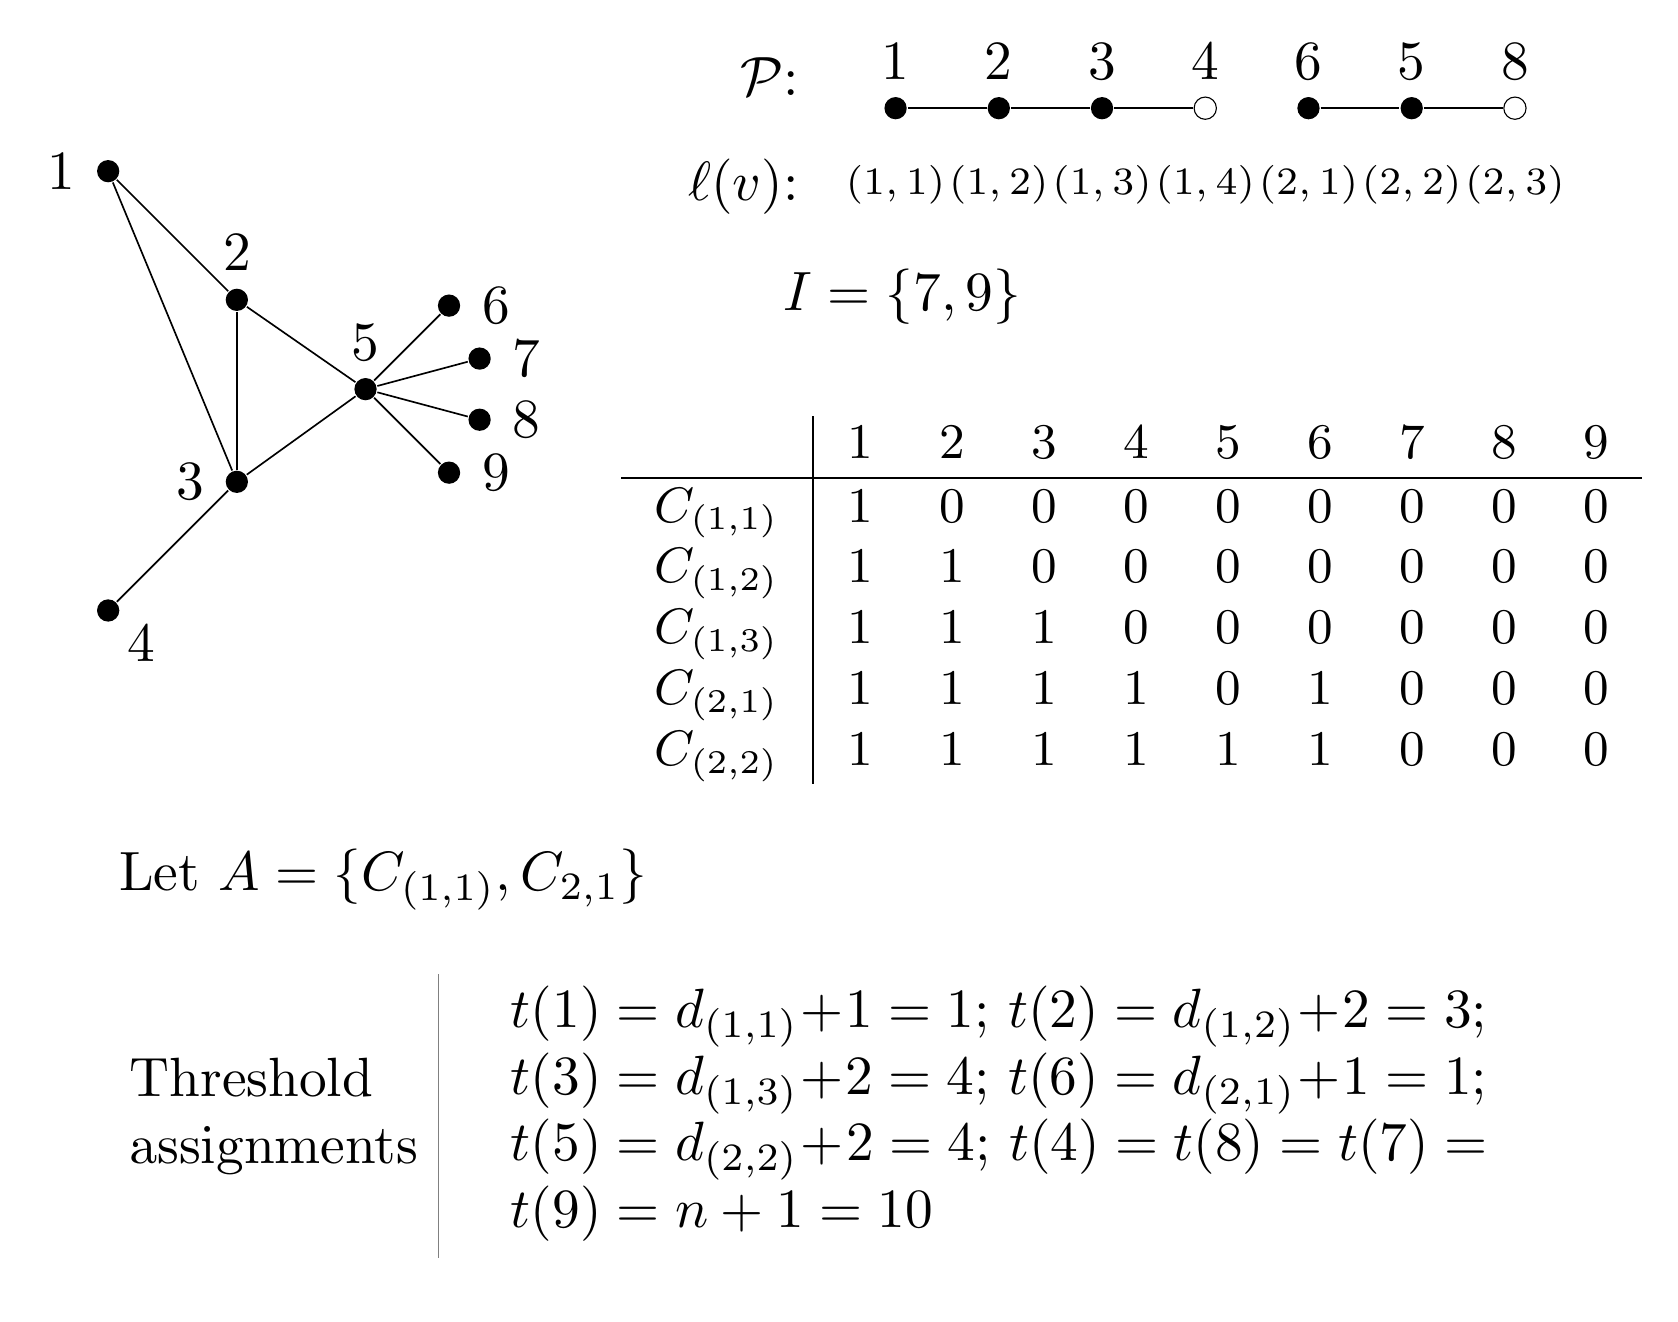
\begin{tikzpicture}
[scale=2,node distance=1cm, transform shape,
every node/.style={shape=circle,fill,inner sep=.5mm},
lab/.style={fill=none},
myedge/.style={>=latex', shorten >=.0pt, shorten <=.0pt,semithick},
subedge/.style={>=latex', shorten >=.0pt, shorten <=.0pt,semithick,black!50},
every fit/.style={fill=black!10,ellipse,draw=black!20},
myellipse/.style={fill=black!20,draw=none}]
%%%%%%%%%%
%%%%% graph
%% vertices
\begin{scope}[shift={(0,0)}]
\node (v1) [label=left:$1$] at (0,0) {};
\node (v2) [label=above:$2$,below right=of v1] {};
\node (v3) [label=left:$3$,below=of v2] {};
\node (v4) [label=below right:$4$,below left=of v3] {};
\node (v5) [label=above:$5$,below right=of v2,shift={(0,.25)}] {};
\begin{scope}[shift={($(v5)$)}]
\def \rad {.75cm}
\node (v6) [label=right:$6$] at ({45}:\rad) {};
\node (v7) [label=right:$7$] at ({15}:\rad) {};
\node (v8) [label=right:$8$] at ({-15}:\rad) {};
\node (v9) [label=right:$9$] at ({-45}:\rad) {};
\end{scope}
%% edges
\draw[myedge] (v1) -- (v2) {};
\draw[myedge] (v1) -- (v3) {};
\draw[myedge] (v2) -- (v3) {};
\draw[myedge] (v2) -- (v5) {};
\draw[myedge] (v3) -- (v4) {};
\draw[myedge] (v3) -- (v5) {};
\draw[myedge] (v5) -- (v6) {};
\draw[myedge] (v5) -- (v7) {};
\draw[myedge] (v5) -- (v8) {};
\draw[myedge] (v5) -- (v9) {};
\end{scope}
%% path decomposition
\begin{scope}[shift={(5,.4)},node distance=.5cm]
\node (v1) [label=above:$1$] at (0,0) {};
\node (v2) [label=above:$2$,right=of v1] {};
\node (v3) [label=above:$3$,right=of v2] {};
\node (v4) [label=above:$4$,right=of v3,fill=none,draw] {};
\node (v6) [label=above:$6$,right=of v4] {};
\node (v5) [label=above:$5$,right=of v6] {};
\node (v8) [label=above:$8$,right=of v5,fill=none,draw] {};
%% edges
\draw[myedge] (v1) -- (v2) {};
\draw[myedge] (v2) -- (v3) {};
\draw[myedge] (v3) -- (v4) {};
\draw[myedge] (v6) -- (v5) {};
\draw[myedge] (v5) -- (v8) {};
%% \draw[subedge] (v1) edge[out=30,in=150] (v3) {};
%% labels
\node [lab,label=below:{\scriptsize $(1,1)$}] at (v1) {};
\node [lab,label=below:{\scriptsize $(1,2)$}] at (v2) {};
\node [lab,label=below:{\scriptsize $(1,3)$}] at (v3) {};
\node [lab,label=below:{\scriptsize $(1,4)$}] at (v4) {};
\node [lab,label=below:{\scriptsize $(2,1)$}] at (v6) {};
\node [lab,label=below:{\scriptsize $(2,2)$}] at (v5) {};
\node [lab,label=below:{\scriptsize $(2,3)$}] at (v8) {};
%% headings
\node [fill=none,anchor=east] at (-.5,.2) {$\mathcal{P}$:};
\node [fill=none,anchor=east] at (-.5,-.5) {$\ell(v)$:};
\node [fill=none,anchor=west] at (-.8,-1.2) {$I=\{7,9\}$};
\end{scope}
%% configurations
\begin{scope}[shift={(3.2,-1.5)},anchor=north west]
\node [draw=none, fill=none, shape=rectangle,scale=1,font=\small] at (0,0) {
   \begin{tabular}{c|ccccccccc}
                             & 1 & 2 & 3 & 4 & 5 & 6 & 7 & 8 & 9 \\\hline
       ${C}_{(1,1)}$ & 1 & 0 & 0 & 0 & 0 & 0 & 0 & 0 & 0 \\
       ${C}_{(1,2)}$ & 1 & 1 & 0 & 0 & 0 & 0 & 0 & 0 & 0 \\
       ${C}_{(1,3)}$ & 1 & 1 & 1 & 0 & 0 & 0 & 0 & 0 & 0 \\
       ${C}_{(2,1)}$ & 1 & 1 & 1 & 1 & 0 & 1 & 0 & 0 & 0 \\
       ${C}_{(2,2)}$ & 1 & 1 & 1 & 1 & 1 & 1 & 0 & 0 & 0 
    \end{tabular}
};
%%    \begin{pgfonlayer}{background}
%%       \draw[myellipse,shift={(-3,.25)}] (0,0) rectangle (6,.35);
%%       \draw[myellipse,shift={(-3,-1)}] (0,0) rectangle (6,.75);
%%    \end{pgfonlayer}
\end{scope}
%% Threshold assignments
\begin{scope}[shift={(0,-4.5)},anchor=north west]
    \node [fill=none,anchor=west] {Let $A=\{C_{(1,1)},C_{2,1}\}$};
    \node [fill=none,text width=2cm,anchor=west] at (0,-1.5) {Threshold assignments};
    \node [shape=rectangle,fill=none,anchor=north west,text width=6.2cm] at
    (2.5,-.62) 
    {$t(1)=d_{(1,1)}+1=1$; $t(2)=d_{(1,2)}+2=3$;
     $t(3)=d_{(1,3)}+2=4$; $t(6)=d_{(2,1)}+1=1$;
     $t(5)=d_{(2,2)}+2=4$; $t(4)=t(8)=t(7)=t(9)=n+1=10$};
\draw[thin,black!50] (2.1,-.6) -- +(0,-1.8);
\end{scope}
\end{tikzpicture}
\end{document}
